\subsection{Implications of the distribution}
Given the latent radius, the conjugate prior for the rate parameter
  $\beta$ is a Gamma distribution, and it is standard practice to assign
  a Gamma distribution to the shape parameter $\alpha$ as well.  We should
  take note, however, what that entails.  In Figure~\ref{fig:prior_implication},
  we see a Gamma$(1,1)^d$ distribution cast to the angular space.  The point of
  this exercise is to ask what shape should we expect to see in the marginal
  $\theta_i$'s, if we assume something along the lines of a uniform prior over
  the unit hypersphere.

\begin{figure}[ht]
  \centering
  \label{fig:prior_implication}
  \title{Independent Gammas Cast to Angular Space}
  \caption{The Marginal density of a Gamma$(1,1)^d$ after casting to angular coordinates.
            The top row is from a two-dimensional the second a three-dimensional,
            the third a four-dimensional, and the bottom a five-dimensional distribution.}
  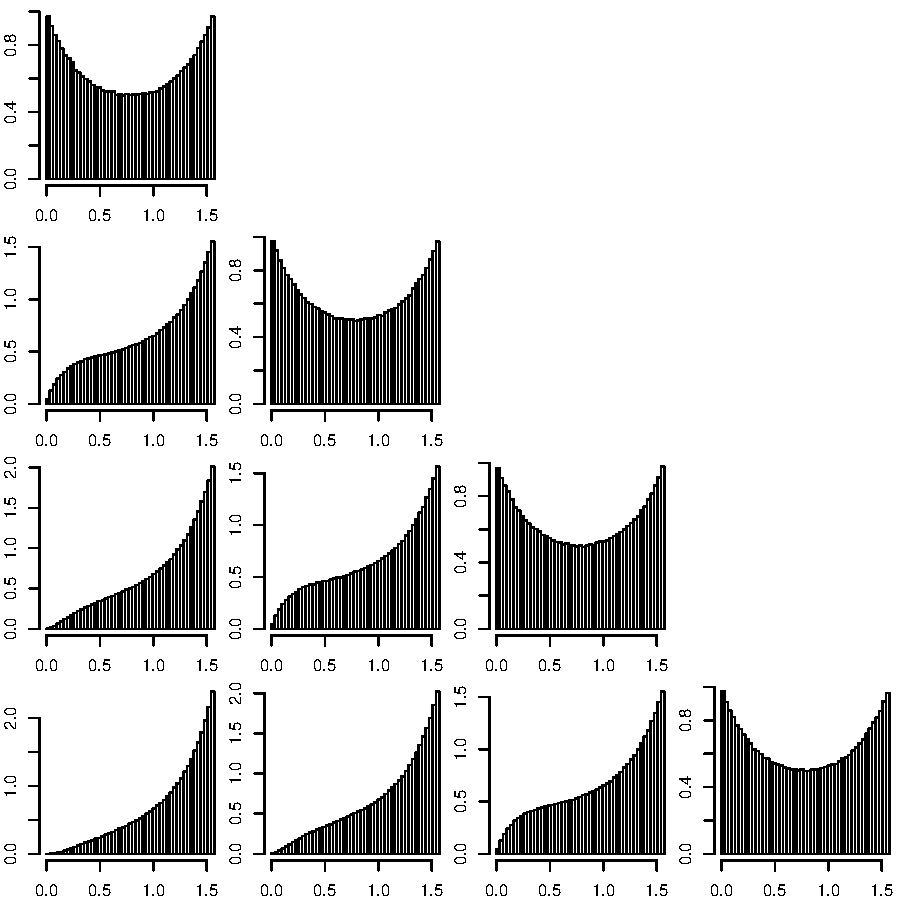
\includegraphics{./images/implication_of_gamma_prior}
\end{figure}

Note that this the resulting distribution of $d$ independent Gamma(1,1) random
  variables, cast to the angular space using Equation~\ref{eqn:invtransform}.  The
  top row represents a two-dimensional gamma distribution, cast to the angular space,
  and every row thereafter increases the dimensionality of the input space by 1.

We see that in the two-dimensional case, the Gamma$(1,1)$ distribution creates a
  density that is biased towards either end of the spectrum, though not excessively.
  There is no combination of gamma distributions that will create a uniform density
  over this space. \makenote{I probably should show this.}  If we extend this space
  to three and more dimensions, we see the distribution of $\theta_1$ through
  $\theta_{d-2}$ shift towards the right, indicating that the mass of the norm of
  a particular observation would tend to fall into the latter columns.  We show this
  here to demonstrate that this is right and expected behavior, so we should expect
  to some degree progressively less right-skewed marginal $\theta_i$ distributions
  when looking at real data.
